\documentclass{standalone}
\usepackage{tikz}
\begin{document}
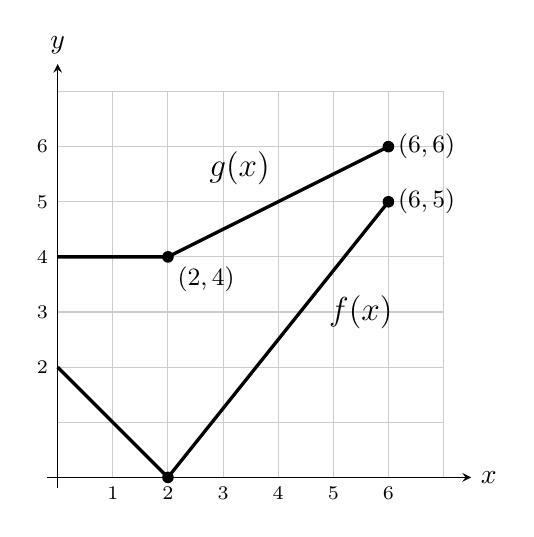
\begin{tikzpicture}[>=stealth, scale=0.7]
  % Light grid
  \draw[gray!40] (0,0) grid (7,7);

  % Axes
  \draw[->] (-0.2,0) -- (7.5,0) node[right] {$x$};
  \draw[<-] (0,7.5) node[above] {$y$} -- (0,-0.2);

  % g(x): (0,4) -> (2,4) -> (6,6), slope 0 then 1/2
  \draw[very thick] (0,4) -- (2,4) -- (6,6);

  % f(x): (0,2) -> (2,0) -> (6,5), slope -1 then 5/4
  \draw[very thick] (0,2) -- (2,0) -- (6,5);

  % Filled dots at labeled points
  \fill (2,4) circle (3pt);
  \fill (6,6) circle (3pt);
  \fill (6,5) circle (3pt);
  \fill (2,0) circle (3pt);

  % Point labels (consistently below and to the right of each point)
  \node[below right,font=\small] at (2,4) {$(2,4)$};
  \node[right,font=\small] at (6,6) {$(6,6)$};
  \node[right,font=\small] at (6,5) {$(6,5)$};

  % Function labels
  \node[font=\large] at (3.3,5.6) {$g(x)$};
  \node[font=\large] at (5.5,3)   {$f(x)$};

  % Axis tick labels
  \foreach \x in {1,2,3,4,5,6} {
    \node[below,font=\scriptsize] at (\x,0) {\x};
  }
  \foreach \y in {2,3,4,5,6} {
    \node[left,font=\scriptsize] at (0,\y) {\y};
  }
\end{tikzpicture}
\end{document}
